\documentclass[preprint,12pt]{elsarticle}
\usepackage{geometry}
%\geometry{letterpaper}                   % ... or a4paper or a5paper or ...
\usepackage{graphicx}
\usepackage{amssymb}
\usepackage{epstopdf} 
%% Use the option review to obtain double line spacing
%% \documentclass[preprint,review,12pt]{elsarticle}

%% Use the options 1p,twocolumn; 3p; 3p,twocolumn; 5p; or 5p,twocolumn
%% for a journal layout:
%% \documentclass[final,1p,times]{elsarticle}
%% \documentclass[final,1p,times,twocolumn]{elsarticle}
%% \documentclass[final,3p,times]{elsarticle}
%% \documentclass[final,3p,times,twocolumn]{elsarticle}
%% \documentclass[final,5p,times]{elsarticle}
%% \documentclass[final,5p,times,twocolumn]{elsarticle}

%% if you use PostScript figures in your article
%% use the graphics package for simple commands
%% \usepackage{graphics}
%% or use the graphicx package for more complicated commands
%% \usepackage{graphicx}
%% or use the epsfig package if you prefer to use the old commands
%% \usepackage{epsfig}

%% The amssymb package provides various useful mathematical symbols
\usepackage{amssymb}
%% The amsthm package provides extended theorem environments
%% \usepackage{amsthm}

%% The lineno packages adds line numbers. Start line numbering with
%% \begin{linenumbers}, end it with \end{linenumbers}. Or switch it on
%% for the whole article with \linenumbers after \end{frontmatter}.
%% \usepackage{lineno}

%% natbib.sty is loaded by default. However, natbib options can be
%% provided with \biboptions{...} command. Following options are
%% valid:

%%   round  -  round parentheses are used (default)
%%   square -  square brackets are used   [option]
%%   curly  -  curly braces are used      {option}
%%   angle  -  angle brackets are used    <option>
%%   semicolon  -  multiple citations separated by semi-colon
%%   colon  - same as semicolon, an earlier confusion
%%   comma  -  separated by comma
%%   numbers-  selects numerical citations
%%   super  -  numerical citations as superscripts
%%   sort   -  sorts multiple citations according to order in ref. list
%%   sort&compress   -  like sort, but also compresses numerical citations
%%   compress - compresses without sorting
%%
%% \biboptions{comma,round}

% \biboptions{}


\journal{Journal of Systems and Software}

%%% OUR MACROS %%%
\newcommand{\COMMENT}[1]{ } 

\begin{document}

\begin{frontmatter}

%% Title, authors and addresses

%% use the tnoteref command within \title for footnotes;
%% use the tnotetext command for the associated footnote;
%% use the fnref command within \author or \address for footnotes;
%% use the fntext command for the associated footnote;
%% use the corref command within \author for corresponding author footnotes;
%% use the cortext command for the associated footnote;
%% use the ead command for the email address,
%% and the form \ead[url] for the home page:
%%
%% \title{Title\tnoteref{label1}}
%% \tnotetext[label1]{}
%% \author{Name\corref{cor1}\fnref{label2}}
%% \ead{email address}
%% \ead[url]{home page}
%% \fntext[label2]{}
%% \cortext[cor1]{}
%% \address{Address\fnref{label3}}
%% \fntext[label3]{}

\title{$\pi$SOD-M: A Methodology for Building Service-Oriented Applications in
the Presence of Non-Functional Properties}

%% use optional labels to link authors explicitly to addresses:
%% \author[label1,label2]{<author name>}
%% \address[label1]{<address>}
%% \address[label2]{<address>} 
 
\author[inst1]{Pl\'acido A. Souza Neto}
\author[inst2]{Genoveva Vargas-Solar}
\author[inst3]{Martin A. Musicante}
\author[inst4]{Valeria~de~Castro}
\author[inst3]{Umberto Souza da Costa}

\address[inst1]{Federal Technological Institute of Rio Grande do Norte -- Natal, Brazil}

\address[inst2]{Universit\'e de Grenoble -- Saint Martin d'H\`{e}res, France}

\address[inst3]{Federal University of Rio Grande do Norte -- Natal, Brazil}

\address[inst4]{Universidad Rey Juan Carlos -- M\'{o}stoles, Spain}

\begin{abstract}
This paper presents\ldots
\end{abstract}

\begin{keyword}
%% keywords here, in the form: keyword \sep keyword

%% MSC codes here, in the form: \MSC code \sep code
%% or \MSC[2008] code \sep code (2000 is the default)

\end{keyword}

\end{frontmatter}

%%
%% Start line numbering here if you want
%%
% \linenumbers

%% main text
%*********************************************************************************************************
\section{Introduction}
\label{sec:intro}

Service oriented computing~\cite{Papazoglou2007} is at the origin of an evolution in the field of software development.
Service oriented methods advocates for the construction of software systems formed by the composition of heterogeneous, loosely coupled modules.
These modules (or services) communicate in order to achieve a common purpose.
 
An important challenge of service oriented development is  to ensure the alignment between the requirements imposed by the business logic and the IT systems actually being developed.
(Moreover, IT systems need to evolve according to the business needs.)
Thus, organizations are seeking for mechanisms to bridge the gap between the actually developed systems and their business needs~\cite{bell}. 
The literature stresses the need for methodologies and techniques for service oriented analysis and design, claiming that they are the cornerstone in the development of meaningful service based applications~\cite{5}.  

In Service-Oriented Computing, pre-existing services are
combined to produce applications and provide the business logic. 
The selection of services is usually guided by the \textit{functional} requirements of the application being developed~\cite{1,2,decastro1,PapazoglouH06}. 
(Functional properties of a computer system are characterized by the effect produced by the system when given a defined input.)
Functional properties are not the only crucial aspect in the software development process. 
Other properties need to be addressed to fit in the application with its context.
These other aspects are called Non-Functional Properties.

Non-functional aspects of the services, often expressed as requirements and constraints in general purpose methodologies, are not usually considered from the early phases of the (service) software process.
Most methods consider them only after the application has been implemented, in order to ensure some level of reliability (e.g., data privacy, exception handling, atomicity, data persistence). 
This leads to service based applications that are partly specified and, thereby, partly compliant with the requirements of the application.
Ideally, non-functional requirements should be considered along with all the stages of the software development. 
The adoption of non-functional specifications from the early states of development
can help the developer to produce applications that are capable of dealing with
the application context.

\bigskip

Model Driven Development (MDD) is a top-down approach for the development of software systems. 
The main ideas of MDD were originally proposed by the Object Management Group (OMG)~\cite{mda}, as a set of guidelines for the structuring of specifications.
The technique advocates for the use of \textit{models} to specify a software system at different levels of abstraction (called \textit{viewpoints}). 
These models are successively refined from abstract specifications into actual computer programs.

In this context, we argue that the convergence of model-driven software development, service orientation and better techniques for documenting and improving business processes are key to make real the idea of rapid, accurate development of software that serves, rather than dictates the needs of its users~\cite{watson}. 

In this work, we are interested in the extension of the \textit{Service Oriented Development Method} (SOD-M)~\cite{decastro1}, to support non-functional aspects, from the early stages of software development.
SOD-M is aligned with the MDD directives and proposes models, practices and techniques for the development of service-based applications.
SOD-M does not provide support for the specification of non-functional requirements, such as
security, reliability, and efficiency. 

The main goals of our work are:
\begin{trivlist}
\item \textit{(i)} To define a NFR model including a set of concepts need for the modeling of NFR in service-oriented applications.
\item \textit{(ii)} To propose a methodology for supporting the construction of service-oriented applications, taking into account both functional and non-functional requirements;
\item \textit{(iii)} To improve the construction process by providing an abstract view of the application and ensure the conformance to its specification;
\item \textit{(iv)} To reduce the programming effort through the semi-automatic generation of  models for the application, to produce concrete implementations from high abstraction models;
\end{trivlist}

The rest of the paper is organized as follows. 
Section\dots






%*********************************************************************************************************

%*********************************************************************************************************
\section{Related Works}
\label{sec:relworks}
%Conceptos existentes en NFR y metodologías similares

Related works to our approach includes existing proposal dealing with the inclusion of non-functional properties in service-oriented development. Standards devoted for expressing non-functional properties for service-oriented applications are also analyzed in this section which needs to be addresses in the code generation phase. Finally exiting methodology for the development of service-oriented applications including non-functional properties are here depicted and compared with our approach.
%As a result of our study of related works, in this section we present a categorization of main concepts related the treatment if non-functional requirement in the field of service-oriented development.

\subsection{Non-functional properties in service-oriented applications}

In previous work we have carried out a systematic review \cite{placidoPhDThesis2012} in order to analyze how non-functional properties are taking into account in existing approaches for service-oriented development. Existing proposals in this field may be classified in three types of works which are described in the followed.

The first types of works are thus considering a particular non-functional concern (e.g. security) which is modeled and then "glued" or associated to functional models of an application. The work of Chollet et al. \cite{CholletL09} defines a proposal to associate non-functional quality properties (security properties in that case) to functional activities which are modeled in a web service composition model.
Schmeling et al. \cite{SchmelingCM11} present an approach and also a toolset for specifying and implementing non-functional concerns in web service compositions; non-functional concerns are modeled first in non-functional model and then related to a service composition represented in a BPMN diagram. Ovaska et al. \cite{OvaskaEHPA10} present an approach to support quality management at design time. Quality requirements are modeled in a first phase and represented then in an architectural model where quality requirements are associated to some components in the model. In our case we propose to model non-functional properties joint to the modeling of functional concerns what simplifies the web service development process. Non-functional properties are represented in our work as constraints and policies but more general quality model such as the proposed by \cite{Goeb2011,Klass2009} could be taken in consideration in further works.

Second type of works related to our proposal proposes specifics architecture or frameworks to manage and validate QoS attributes in service composition processes. The work of Xiao et al. \cite{XiaoCZBOLH08} present a framework to verify SLA compliance in composed services. Task in a BPEL process can be annotated with non-functional attributes (such as time, cost, resources, etc.) which are validated at design time. A similar work is presented in \cite{SchmelingCM11} by using a formal method that allows to choice best suited services instances according to a service composition pattern that include some QoS attributes. Babamir et al. present in \cite{Babamir2010} a framework for evaluate quality attributes of web services. By executing an algorithm, the framework allow to choice best web services for any task in a process and also candidate web service to replace original ones in cases it cannot perform at runtime. In \cite{Karunamurthy2012787} authors propose architecture in which web services may be described with non-functional characteristics that are validated in the service composition process.

Third type of works include proposal working on the evaluation and matching of non-functional properties in the process of search or invocation of particular web services.\cite{AgarwalLS09} define a policy language that provides a way to specific constraints on functional as well as non-functional properties of Web services with the aim of facilitating automated discovery and selection of services.\cite{JeongCL09,Kamalabad2012} defines also proposals to the validate quality attributes of web services when discover and compose.\cite{MohantyRP10} works also on the selection of web service for use considering non-functional properties. The paper present web services quality prediction models, which take non-functional properties into account. Similarly, \cite{Yeom2006} define a quality driven selection of web services providing a QoS model.

Our proposal by the contrary to the second and third type of proposals is focusing on the design of service-oriented application with non-functional properties and not on the validation of QoS attributes at runtime.

Other relevant works such as \cite{DAmbrogio06,Liu20121080} propose extensions to WSDL and BPEL languages respectively for the inclusion of QoS attributes that can be evaluated at runtime.

\subsection{Standards for programming non-functional properties in service-oriented applications}

Current standards in services' composition implement functional, non-functional constraints and communication aspects by combining different languages and protocols. WSDL and SOAP among others are languages used respectively for describing services' interfaces and message exchange protocols for calling methods exported by such services. For adding a transactional behaviour to a services' composition it is necessary to implement WS-Coordination, WS-Transaction, WS-BussinessActivity and WS-AtomicTransaction. The selection of the adequate protocols for adding a specific non-functional constraints to a services' composition (e.g., security, transactional behaviour and adaptability) is responsibility of a programmer. As a consequence, the development of an application based on a services' composition is a complex and a time-consuming process. This is opposed to the philosophy of services that aims at facilitating the integration of distributed applications. Other works, like \cite{Fauvet05} introduce a model for transactional services composition based on an advanced transactional model.\cite{BhiriGP05} proposes an approach that consists of a set of algorithms and rules to assist designers to compose transactional services. In \cite{Vidyasankar:2004} the model introduced in \cite{SchuldtABS02} is extended to web services for addressing atomicity.

As WS-* and similar approaches, our work enables the specification and programming of crosscutting aspects (i.e., atomicity, security, exception handling, persistence).
In contrast to these approaches, our work specifies policies for a services' composition in an orthogonal way. Besides, these approaches suppose that non-functional properties are implemented according a the knowledge that a programmer has of a specific application requirements but they are not derived in a methodological way, leading to ad-hoc solutions that can be difficult to reuse. In our approach, once defined the policies for a given application they can be reused and/or specialized for another one with the same requirements or that uses services that impose the same constraints.

\subsection{Methodologies for Service-oriented applications development including non-functional properties}

Beside the works presented above, there are few methodologies for service-oriented development that address the explicit modeling of non functional properties for service-based applications. Important methodologies for building service-based applications have been proposed in the last years \cite{Ramollari_asurvey,PapazoglouH06,FeuerlichtM05,soma,Arsanjani:2008}, but all of they focus mainly on the modeling and construction process of service-based business processes that represent the functionally of information systems.

Some methodologies dealing with particular non-functional properties in service orientation have also appeared. Tran et al. \cite{Tran2012531} present a model-driven approach for addressing problems related to compliance concerns. Authors define extend elements of a business process models with elements of a compliance model in which QoS policies are represented.\cite{GutierrezRF10} present PWSSec process, a methodology that provide developers with all the activities, tasks, tools, security artifacts and organizational structures necessary to design a secure WS-based solution.

Unlike methodologies and approaches providing best practices presented above, the main contribution of our proposal is that, integrated to a method that allows to model service-based applications starting from a high-level business modelling, and defining meta-models at different abstraction levels (CIM, PIM and PSM), it enables the design and development of services-based applications that can be reused and that are reliable. The definition of a model-driven approach that allows to model non-functional properties in the early stages of the software development process, and the definition of model transformations to go down in the development process adding more a more implementation details at each modelling stage is a key benefits of our proposal.

%\textit{Design by Contract} \cite{HL05TACoS} is an approach for specifying web services and verifying them through runtime checkers before they are deployed. A contract adds behavioral information to a service specification, that is, it specifies the conditions in which methods exported by a service can be called. Contracts are expressed using the language \textit{jmlrac} \cite{LeavensCCRC02}. The \textit{Contract Definition Language} (CDL) \cite{cdl2006} is a XML-based description language, for defining contracts for services. There are an associated architecture framework, design standards and a methodology, for developing applications using services.  A services' based application  specification is generated after several \cite{AbrialLNSS91} B-machines refinements that describe the services and their compositions.

%\cite{PapazoglouH06} proposes a methodology based on a SOA extension. This work defines a service oriented business process development methodology with phases for business process development. The whole life-cycle is based on six phases: planning, analysis and design, construction and testing, provisioning, deployment, and execution and monitoring.
%IBM proposes a methodology for the development of SOA solutions, called SOMA \cite{soma}. SOMA defines a life-cycle with seven phases: business modeling and transformation, solution management, identification,
%specification, realization, implementation and deployment monitoring and management.

%\cite{sommerville08} describes some key points for building services' based applications based on business process models that define the activities and information exchanged in a business processes. Activities in business process can be performed by services so that the model of business process
%represents a composition of services. It classifies services   as public utilities, business services or
%composition services. Software development that uses services involves creating programs for composing and configuring services to create new composite services. The service engineering process involves identifying services candidates, service interface and implementation definition, testing and deployment of each service.







\subsection{Modeling non-functional requirements in service-oriented applications}
\label{sec:modeling}
%(comentar la revisión y presentar la clasificacion de conceptos y NFR model con los conceptos que proponemos) 
%(comentar la revisión y presentar la clasificacion de conceptos y NFR model con los conceptos que proponemos)
% De Valeria: Lo he quitado porque no sé si tiene mucho sentido hacerlo aquí. Quizás ponemos el pequeño modelo que hicimos con los conceptos ya en la sección del método.  

\subsection{Methodologies for Service-oriented applications development including non-functional requirements}
\label{sec:methodologies}
%(aqui propuestas relacionadas, analizar sus caracteristicas, si son MDD, si parte de alto nivel, etc.)
%(aqui propuestas relacionadas, analizar sus caracteristicas, si son MDD, si parte de alto nivel, etc.)

Model Driven Development (MDD)~\cite{mda} is a top-down approach for the development of software systems. 
MDD uses the notion of \textit{model} to specify a software system at different levels of abstraction (called \textit{viewpoints}):

\begin{trivlist}
\item \textbf{Computation Independent Models (CIM):} This level focusses on the
environment of the system, as well as on its business and requirement specifications. 
This viewpoint represents the software system at its highest level of abstraction. 
At this moment of the development, the structure and system processing details are still unknown or undetermined. 
 
\item \textbf{Platform Independent Models (PIM):} This level focusses on the system functionality, hiding the details of any particular platform. 
The specification defines those parts of the system that do not change from one platform to another. 

\item \textbf{Platform Specific Models (PSM):} This level focusses on the functionality, in the context of a particular implementation platform.
Models at this level combine the platform-independent view with the specific aspects of the platform to implement the system.  
\end{trivlist}

Besides the notion of model at each level of abstraction, MDD requires the use of \textit{model transformations} within and between levels.
Intra-level transformations are used to provide a unified representation of concepts of a given level.
Inter-level transformation implement a refinement process between levels.
Transformations may be automatic or semi-automatic.



%*********************************************************************************************************

%*********************************************************************************************************
\section{Modeling reliable services' compositions with $\pi$-SOD-M}\label{sec:motivation}
%(Aquí lo dejaría con la estructura que teníamos para Caise, presentamos el framework y posteriormente comentamos modelos y transformaciones)

In this section we present $\pi$SOD-M, an MDD based methodology.
$\pi$SOD-M provides an environment for building service compositions.
$\pi$SOD-M includes the modelling of non-functional requirements at the early stages of the development.
The methof extends the SOD-M meta-models by adding the concept of \textit{Policy}~\cite{Espinosa-Oviedo2011a} to represent non-functional requirements.

\begin{figure}[h]
\centering
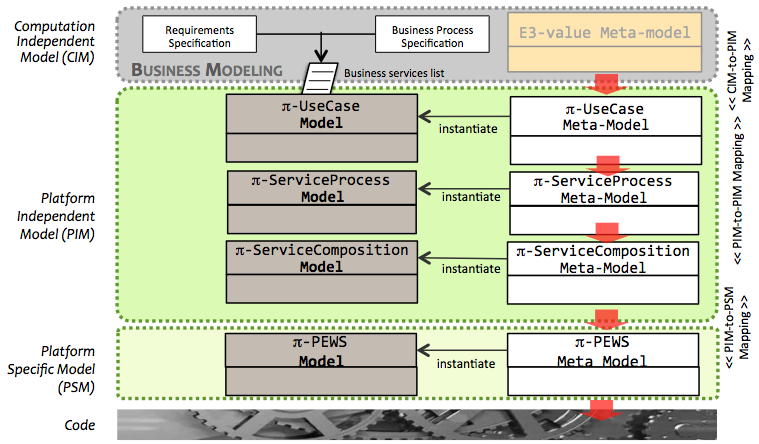
\includegraphics[width=1.0\textwidth]{figs/piSODM}
\caption{$\pi$SOD-M Overview.}
\label{fig:piSOD-M}
\end{figure}

$\pi$SOD-M (Figure~\ref{fig:piSOD-M}) proposes the generation of a set of models at different levels of abstraction, as well as transformations between these models.
$\pi$SOD-M models represent both the functional aspects of the application as well as its non-functional constraints.
Constraints are restrictions that must be verified during the execution of the application.
An example of this is the requirement of the user's authentication for executing some system functions.

Similarly to SOD-M, our approach targets the construction of service-oriented applications that implement business processes.
$\pi$SOD-M proposes a development process based on the definition of models (instances of the meta-modes) and transformations between models.
There are two kinds of transformations: Model-to-model transformations are used during the software process to refine the specification.
Model-to-text transformations are the last step of the process and generate code.

We extend SOD-M to include non-functional specifications.
Our method defines four meta-models: \textit{$\pi$-UseCase}, \textit{$\pi$-ServiceProcess}, \textit{$\pi$-ServiceCom\-po\-si\-tion} and \textit{$\pi$-PEWS}.
The former three are extensions of SOD-M meta-models and belong to the PIM level.
The \textit{$\pi$-PEWS} meta-model is a PSM.

The \textit{$\pi$-UseCase} meta-model describes functional and non-functional requirements.
Non-functional requirements are defined as \textit{constraints} over processing and data.
The \textit{$\pi$-ServiceProcess} meta-model defines the concept of \textit{service contract} to represent restrictions over data and actions that must be performed upon certain conditions.
The \textit{$\pi$-ServiceProcess} meta-model gathers the constraints
described in the \textit{$\pi$-UseCase} model into contracts that are associated
with services.
The \textit{$\pi$-ServiceComposition} meta-model provides the concept of \textit{Policy}
which put together contracts with similar non-functional requirements.
For instance, security and privacy restrictions may be grouped into a security policy.
\textit{$\pi$-ServiceComposition} models can be refined into PSMs.

At the PSM level we have lower-level models that can be automatically translated into actual computer programs.
The \textit{$\pi$-PEWS} meta-model is the PSM adopted in this work.
\textit{$\pi$-PEWS} models are textual descriptions of service compositions that can be translated into any service composition language, such as BPEL~\cite{bpel03} or PEWS~\cite{BaCAM05,Placido2010LTPD}.
This can be accomplished by defining: \textit{(i)} a model-to-model transformation, from a \textit{$\pi$-ServiceComposition} model to the corresponding PSM, and \textit{(ii)} a model-to-text transformation, from the this PSM to the composition language.

%(Aquí lo dejaría con la estructura que teníamos para Caise, presentamos el framework y posteriormente comentamos modelos y transformaciones)

\subsection{$\pi$-SOD-M meta-models}\label{sec:pisodmmetamodels}
%3.1. pi-SoD-M metamodels (presentar los metamodels)
%3.1. pi-SoD-M metamodels (presentar los metamodels)

Extending from the highest level of abstraction of the MDA, $\pi$-SODM provides  a conceptual structure to: first, capture the system requirements and specification in high-level abstraction models (computation independent models, CIMs); next,  starting from such models build platform independent models (PIMs) specifying the system details; next transform such models into platform specific models (PSMs) that bundles the specification of the system with the details of the targeted platform; and finally, serialize such model into code that implements the system. 

\subsubsection{Computation Independent Models}
$\Pi$-SODM uses two models at the CIM level: The E3value~\cite{e3value} model and BPMN~\cite{BPMN}.
The former  identifies the transference of value information between components of the system.
The BPMN model establishes which are the actors and main tasks of the application.

The e3value defines \textit{dependency paths}, showing the value exchanges, which are triggered by the occurrence of an end-consumer need (in our case, the need of a risk assessment). 
A dependency path has a direction and consists of a sequence of linked dependency nodes.
A dependency path starts with a \textit{start stimulus} node and ends with an \textit{end stimulus} node\footnote{See Legend on Figure~\ref{fig:E3valuemodel}}. 
Dependency paths may also contain \textsl{OR} and \textsl{AND} elements (both for initiate and join alternative and parallel paths).

\subsubsection{Platform Independent Models}
 The \textit{$\pi$-UseCase} meta-model extends the UML Use Case meta-model for describing functional and non-functional requirements. Non-functional requirements are defined as \textit{constraints} over actions and data.
 
The \textit{$\pi$-ServiceProcess} meta-model defines the concept of \textit{service contract} to represent constraints over data and actions 
%that must be performed upon certain conditions.
%The \textit{$\pi$-ServiceProcess} meta-model gathers the constraints
described in the \textit{$\pi$-UseCase}.
%model into contracts that are associated
%with services.

The \textit{$\pi$-ServiceComposition} meta-model provides the concept  \textit{Policy}
to integrate contracts with similar non-functional requirements.
For instance, security and privacy restrictions may be grouped into a security policy.
%\textit{$\pi$-ServiceComposition} models can be refined into PSMs.



\subsubsection{Platform Specific Models}

The \textit{$\pi$-PEWS} meta-model provides concepts for modelling service compositions. 
Instances of this meta-model are textual descriptions of service compositions that can be translated into any service composition language, such as BPEL~\cite{bpel03} or PEWS~\cite{BaCAM05,Placido2010LTPD}.

PEWS~\cite{BHM06,Placido2010LTPD} is a notation to express service compositions.
The language is based on the notion of Path Expressions~\cite{And79} and can easily be translated into any actual composition language, such as BPEL~\cite{bpel03} or any other language that lets the service designer combine the methods or subprograms that implement each operation of a service, in order to achieve the desired application logic. 
Figure~\ref{fig:metamodel} presents the $\pi$-{\sc Pews} meta-model, where we identify classes to describe:
\begin{itemizedTrivlist}
\item Service compositions: {\sc Namespace} representing the interface exported by a service, {\sc Operation} that represents a call to a service method, {\sc CompositeOperation}, {\sc Operator} and {\sc Path} for representing service compositions.
A {\sc Path} can be an {\sc Operation} or a {\sc Compound Operation}. 
A {\sc Compound Operation} is defined using an {\sc Operator}.
The language defines operators to denote guarded operations ($[C]S$); sequential ($\ . \ $), parallel ($\ \| \ $) and alternative ($\ + \ $) compositions; as well as sequential ($*$) and parallel ($\{\dots\}$) repetition.

\item {\em A-Policies} that can be associated to a service compositions:  {\sc A-Policy}, {\sc Rule}, {\sc Event}, {\sc Condition}, {\sc Action}, {\sc State}, and {\sc Scope}.
A brief description of these classes is given next.
\end{itemizedTrivlist}
%
\begin{figure}[t]
\centering
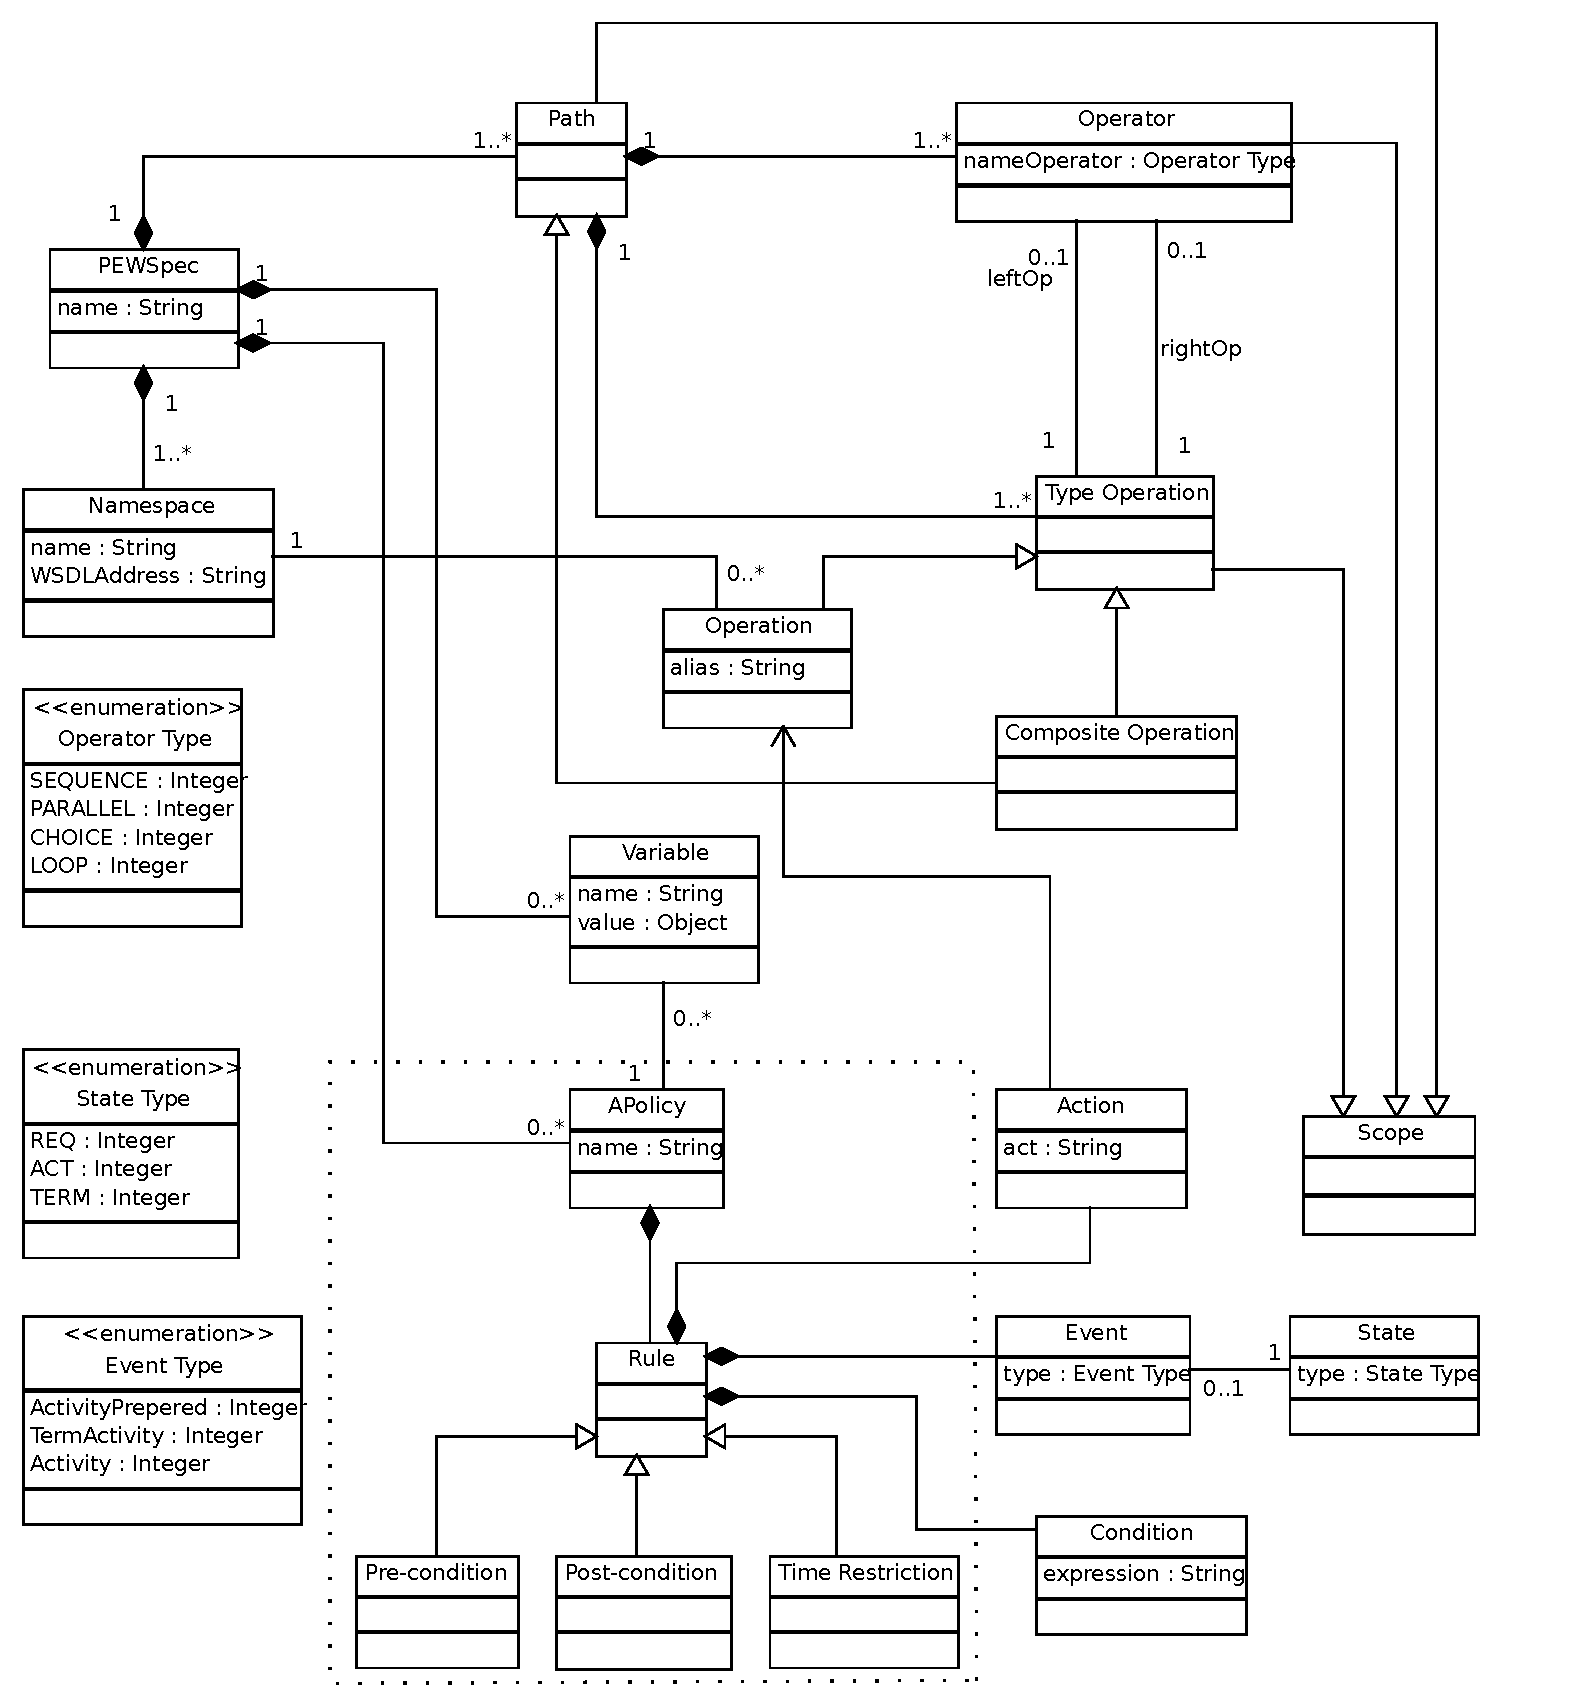
\includegraphics[width=1.0\textwidth]{figs/PEWSMetamodel}
\caption{$\pi$-{\sc Pews} Metamodel}
\label{fig:metamodel}
\end{figure}

Figure~\ref{fig:metamodel} shows that each {\sc A-Policy} is associated to a {\sc Scope} that can be either an {\sc Operation} (e.g., an authentication protocol associated to a method exported by a service),  an {\sc Operator} (e.g., a temporal constraint associated to a sequence of operators) or a {\sc Path}.  
Each {\sc A-Policy} groups a set of ECA rules with a classic semantics, i.e, {\em when an event of type E occurs, if condition C is verified then execute the action A}.  
In this way, an {\em A-policy} represents a set of reactions to be possibly executed when one or several events are notified.
%In this way,
%\begin{itemizedTrivlist}
%\item The class {\sc Scope} represents any element of a service composition (i.e., operation, operator, path).
%\item The class {\sc A-Policy} represents a recovery strategy implemented by ECA rules of the form {\sc Event} - {\sc Condition} - {\sc Action}. 
%An {\em A-policy} has variables that represent the view of the execution state of its associated scope, that is required for executing the rules. The value of a variable is represented using the type {\sc Variable}. The class {\sc A-Policy} is specialized for defining specific constraints, for instance authentication {\em A-policies}.
%\end{itemizedTrivlist}
%
%An authentication {\em A-policy} represents the situation where an invocation in
%an activity occurs until its sender and/or its recipient have been
%identified. Typically, authentication A-Policies ensure that the invocation of the activity will be done within an authentication protocol.

Given a $\pi$-SCM model of a specific service based application (expressed according to the $\pi$-SCM meta-model), it is possible to generate its corresponding $\pi$-{\sc Pews} model. 
The following section describes the transformation rules between the $\pi$-SCM and $\pi$-{\sc Pews} meta-models.






===================================

The {\em A-policy} based service composition ($\pi$-SCM) meta-model, shown in Figure \ref{fig:e-scomposition-metamodel},
provides meta-classes to represent workflows\footnote{Workflows will be transformed into implemented service compositions.} that model  business processes.
The meta-model identifies {\sc Business Collaborators}\footnote{We use {\sc capitals} for referring to meta-model meta-classes.} and the {\sc Actions} they perform. 
Instances of this meta-model are represented as UML activity diagrams. 
In Figure~\ref{fig:e-scomposition-metamodel}  coloured boxes illustrate classes  modelling  non-functional properties and 
 white boxes represent classes modelling functional ones. 

%In the meta-model of Figure~\ref{fig:e-scomposition-metamodel}:
\begin{itemizedTrivlist}
\item A {\sc Business Collaborator} meta-class represents the classes of entities that collaborate in  business processes by performing some  required action. 
An instance of this meta-class is graphically represented as a partition in the activity diagram. 
A collaborator can be either internal or external to the system. 
When the collaborator of the business is external to the system, the attribute {\sf IsExternal}\footnote{We use the {\sf sans serif} font for referring to classes defined using a meta-model.} of the collaborator is set to \textbf{true}.

\item {\sc Action}s, a kind of {\sc ExecutableNode}, are represented in the model as a class activity instance of the meta-class Action. 
A class action represents some type of transformation or processing. 
There are two types of actions: i) a WebService (attribute Type is {\sf WS}); and ii) a simple operation called an {\sc ActivityOperation} (attribute Type is {\sc AOP}).
\begin{figure}[t]
\centering
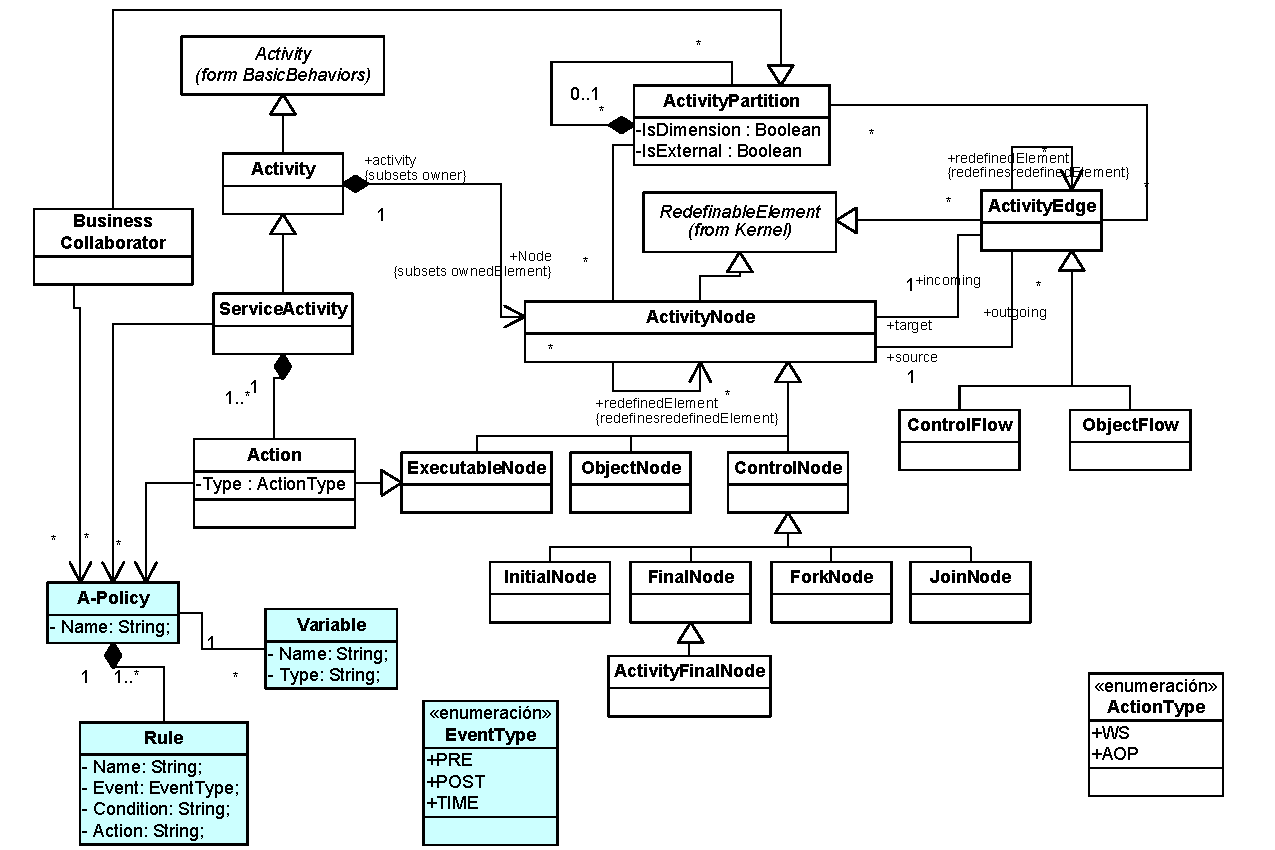
\includegraphics[width=1.0\textwidth]{figs/E-service-composition-metamodel}
\caption{$\pi$-Service Composition ($\pi$-SCM) Metamodel.}
\label{fig:e-scomposition-metamodel}
\end{figure}

\item The {\sc ServiceActivity} meta-class represents classes of composite activity types that must be carried out as part of a business service and is composed by one or more executable nodes.

\item In order to represent constraints types associated to services compositions, we extended introduced the meta-classes {\sc Rule} and {\sc A-policy} (see blue meta-classes in the $\pi$-SCM meta-model in Figure \ref{fig:e-scomposition-metamodel}).
We model non-functional constraints by using the notion of {\em A-policy}~\cite{Espinosa-Oviedo2011a,CIC:eovszmc09c}.
An {\em A-policy} is defined by attributes and rules. 
Intuitively, the conditions of each rule will be checked.
In case of no compliance, the actions defined by the rule will be performed.
The {\sc Rule} meta-class represents the types of event - condition - action rules where the {\sc Event} part represents the moment in which a constraint  will be evaluated.
An {\em A-policy} defines variables and operations that can be shared by the rules and that can be used for expressing their Event and Condition parts. 
\end{itemizedTrivlist}

\begin{figure}[t]%[htpb]
\centering
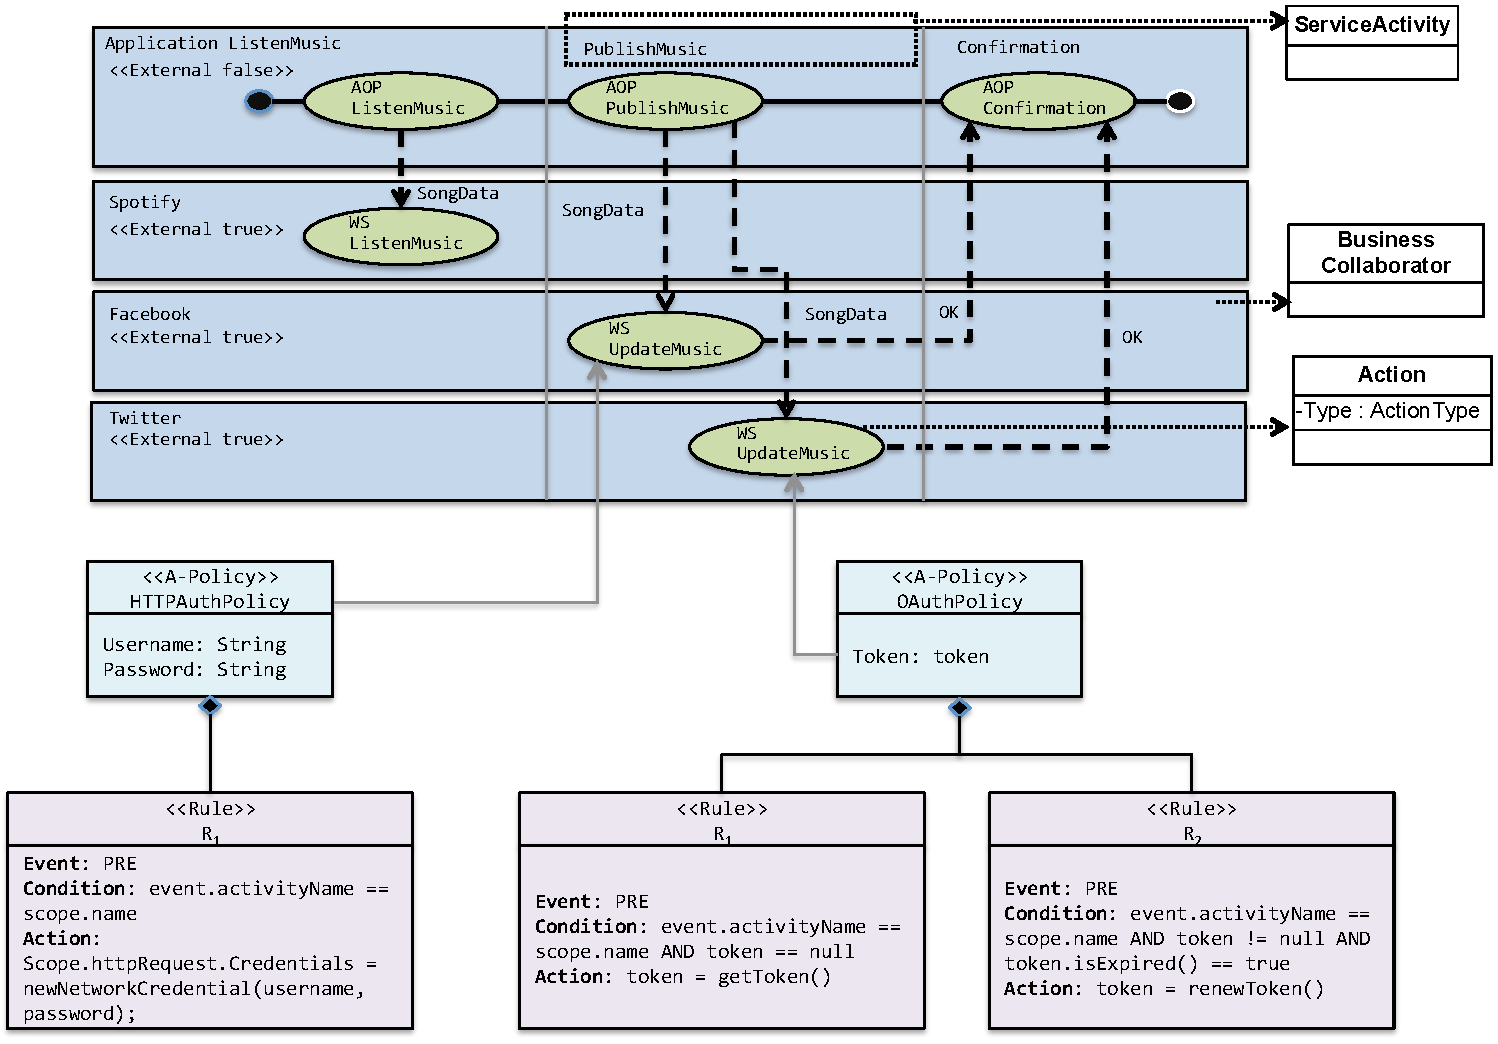
\includegraphics[width=0.95\textwidth]{figs/e-composition-model}

{\color{red}\LARGE PLACIDO: Please change the names of the boxes in accordance to the explanation --Martin}

\caption{$\pi$-SCM for the ``To publish music'' business service.}
\label{fig:servicecompositionmodel}
\end{figure}

\begin{example}[To Publish Music]\label{ex:toPublicMusic}
To illustrate the use of the $\pi$-Service Composition Meta-model, we define a model for the ``To Publish Music'' scenario (Figure \ref{fig:servicecompositionmodel}). 
In this model, there are three external business collaborators ({\em Spotify, Twitter} and {\em Facebook}).
% \footnote{We use {\em italics} to refer to concrete values of the classes of a model that are derived from the classes of a meta-model.}). 
The model also shows the business process of the application that consists of three service activities: {\em Listen Music}, {\em Public Music} and {\em Confirmation}. 
Note that  the activity {\em Publish Music} calls the actions of two service collaborators namely {\em Facebook} and {\em Twitter}.
Both {\em Facebook} and {\em Twitter} services require authentication protocols in order to execute methods that will read and update the user space. 
%A call to such services must be part of the authentication protocol required by these services.
In the example we  associate two authentication policies, one for the open authentication protocol, represented by the class {\sf\small OAuthPolicy} at {\em Twitter}, that will be associated to the activity  {\sf\small UpdateTwitter} (see Figure \ref{fig:servicecompositionmodel}). 
In the same way, the {\em Facebook} class {\sf\small HTTPAuthPolicy}, for the http authentication protocol will be associated to the activity {\sf\small UpdateFacebook}.

{\sf\small OAuthPolicy} will implement the open authentication protocol.
The {\em A-policy} {\sf\small OAuthPolicy} has a variable {\sf\small Token} that will be used to store the authentication token provided by the service.
This variable is imported through the library {\sf\small OAuthPolicy.Token}. 
The A-policy {\sf\small OAuthPolicy} defines two rules, both can be triggered by events of type {\sf\small ActivityPrepared}: (R$_1$): If no token has been associated to the variable {\sf\small token}, then a token is obtained ; and (R$_2$): if the token has expired, then it is renewed. 
Notice that the code in the actions profits from the imported {\sf\small OAuthPolicy.Token} for transparently obtaining or renewing a token from a third party.

{\sf\small HTTPAuthPolicy} implements the HTTP-Auth protocol. 
The A-policy imports an http protocol library and it has two variables {\sf\small username} and {\sf\small password}.  
The event of type {\sf\small ActivityPrepared} is the triggering event of the rule {\sf\small R$_1$}. 
On the notification of an event of that type, a credential is obtained using the username and password. 
\hfill\openbox
\end{example}

We propose the use of rules and policies to model and associate non-functional properties to service compositions.
These artifacts will be used to generate the actual programs that will implement the application:
Once the $\pi$-Service Composition Model has been defined, then it can be transformed into a lower level model (in our case, $\pi$-PEWS) that gives support to code generation. 
The $\pi$-PEWS  meta-model is described in the next section. 


%..--..--..--..--..--..--..--..--..--..--..--..--..--..--..--..--..--..--..--..--..--..--..--..--..--..--..--..--..--..--..--..
\subsubsection{$\pi$-{\sc Pews}  meta-model}\label{sec:pewsmetamodel}
%..--..--..--..--..--..--..--..--..--..--..--..--..--..--..--..--..--..--..--..--..--..--..--..--..--..--..--..--..--..--..--..






\subsection{$\pi$-SOD-M transformations}\label{sec:pisodmtransformations}
%3.2. pi-sod-M transformations (con la tablas del caise)

Figures~\ref{fig:transformationsA}, \ref{fig:transformationsB} and \ref{fig:transformationsC} show the transformation rules from the elements of a $\pi$-SCM meta-model into elements of the $\pi$-{\sc Pews} meta-model. 
There are two groups of rules: those that transform service composition elements of the $\pi$-SCM to $\pi$-{\sc Pews} meta-models elements; and those that transform rules grouped by policies into {\em A-policy} types.
\begin{figure}
\centering{
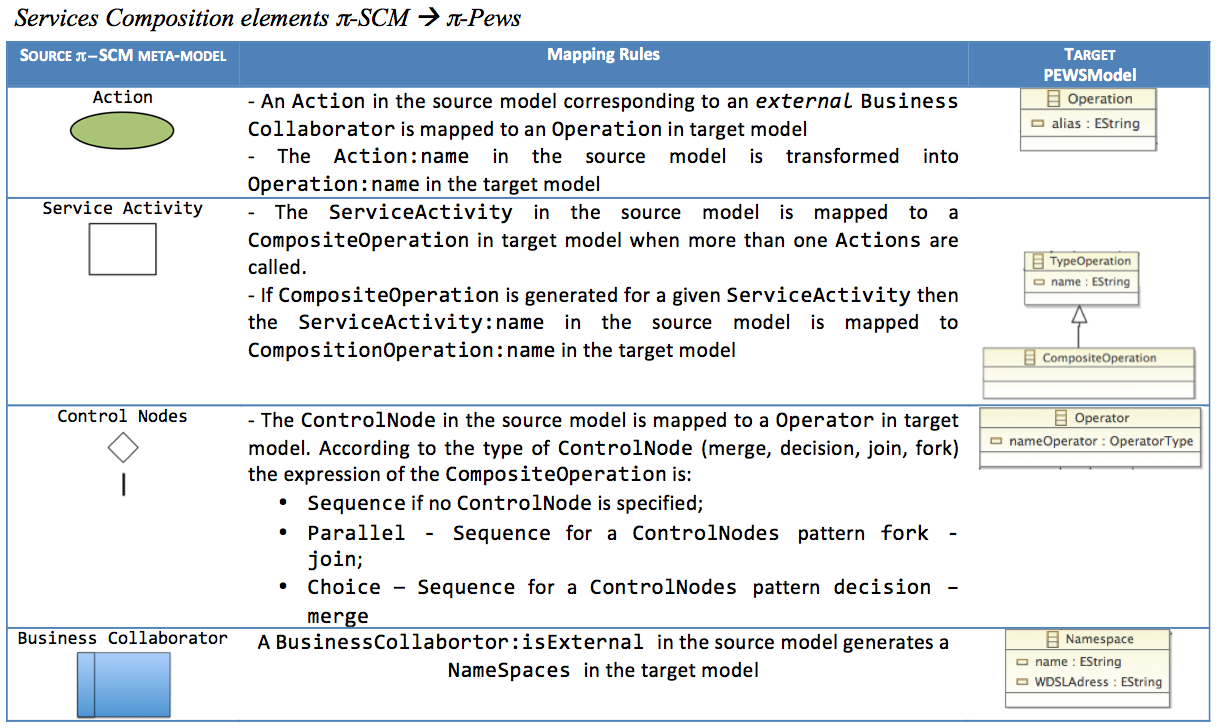
\includegraphics[width=0.96\textwidth]{figs/Mapping-1a.png}
}
\caption{ $\pi$-SCM to $\pi$-{\sc Pews} transformations (Services).}
\label{fig:transformationsA}
\end{figure}


\subsection{Transformation of $\pi$-SCM service composition elements into $\pi$-{\sc Pews} elements}

The transformation rules concerning service composition elements of $\pi$-SCM are shown in figure~\ref{fig:transformationsA}.
Named actions of $\pi$-SCM (represented by {\sc\em Action} and {\sc\em Action:name}) are transformed into a named class {\sc Operation} with a corresponding attribute name {\sc Operation:name}. 
Named service activities represented by the elements {\sc\em ServiceActivity}  and  {\sc\em ServiceActivity:name} of the $\pi$-SCM are transformed into named operations of the $\pi$-{\sc Pews} model, represented by the elements {\sc CompositeOperation} and {\sc CompositeOperation:name}. 
Workflow definitions are translated to the usual control flow structures, using the sequential, parallel and choice combinators of PEWS.

\begin{example}
In the scenario ``To Publish Music'' of Example~\ref{ex:toPublicMusic}, the service activity {\sf PublishMusic} of the $\pi$-SC model calls to two {\sf Activities} of type {\em UpdateMusic}, respectively concerning the {\em Facebook} and {\em Twitter} business services. 
The {\sf Composite Operation} named {\em PublishSong} of the $\pi$-{\sc Pews} model is obtained.
This operation uses the parallel constructor and it is written: {\sf PublishFacebook} $\parallel$ {\sf PublishTwitter}.
\end{example}



\subsection{Transformation of A-policies and rules into $\pi$-{\sc Pews}}

The {\em A-policies} defined for the elements of $\pi$-SCM are transformed into $\pi$-{\sc Pews} {\sc A-Policy} classes.
These classes keep their names, as expressed in the source model. 
The transformation of \textit{rules} is guided by the event types associated to these rules.
The $\pi$-SCM {\em A-policy} variables, given as {\sc\em $<$Variable:name, Variable:type$>$} are transformed into elements of type {\sc Variable} with attributes {\sc name} and {\sc type} of the $\pi$-SCM model.

As shown in Figures~\ref{fig:transformationsB} and~\ref{fig:transformationsC}, for an event of type {\sc\em Pre} the corresponding transformed rule is of type {\sc Precondition}; for an event of type {\sc\em Post} the corresponding transformed rule is of type {\sc Postcondition}; finally, for an event of type {\sc\em TimeRestriction} the corresponding transformed rule is of type {\sc Time}. 
The condition inside a $\pi$-SCM rule ({\sc\em Rule:condition}) is transformed into a class {\sc\em Condition:expression} where the attributes of the expression are transformed into elements of type {\sc Attribute}.

\begin{figure}
\centering{
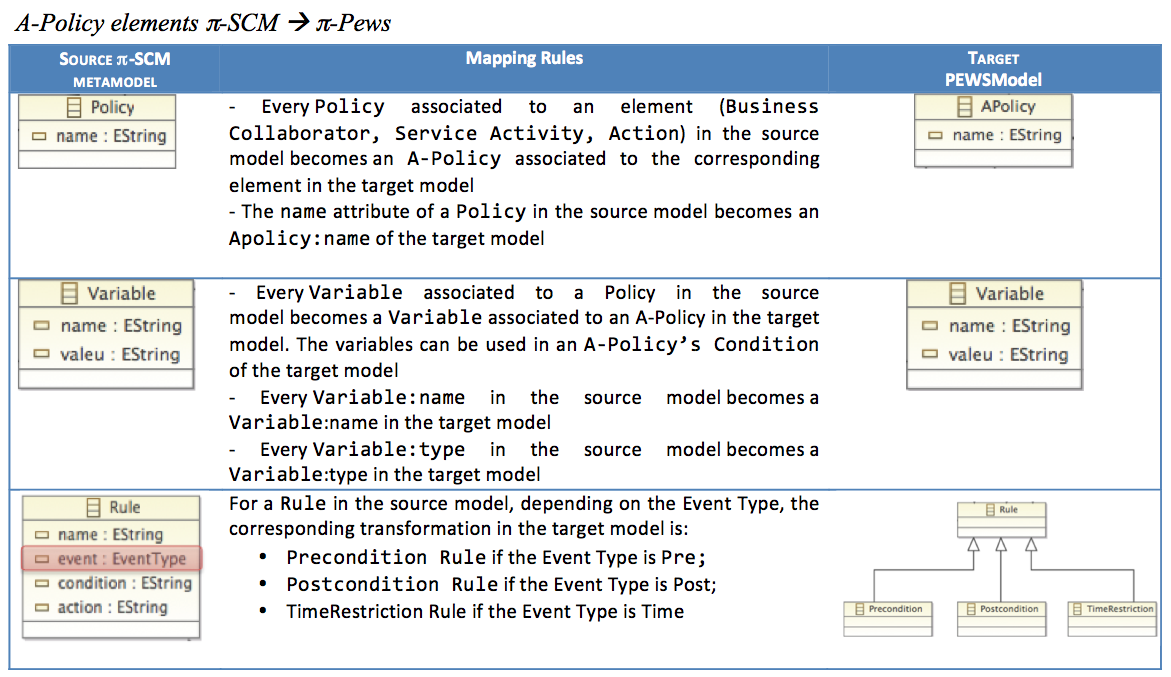
\includegraphics[width=0.96\textwidth]{figs/Mapping-1b.png}
}
\caption{ $\pi$-SCM to $\pi$-{\sc Pews} transformations (\textit{A-Policies}).}
\label{fig:transformationsB}
\end{figure}

\begin{example}
In the ``To Publish Music'' scenario of Example~\ref{ex:toPublicMusic}, the {\sf Policies} {\em OAuthPolicy} and {\em HTTPAuthPolicy} of the $\pi$-SCM model are transformed into {\em A-policies} of type {\sf Precondition} of the $\pi$-{\sc Pews} model. 
In both cases the events are of type {\sf ActivityPrepared}. 
These policies, as stated in the $\pi$-SCM model, are associated to {\sf Activities}. 
Their transformed counterparts are associated to operations {\em PublishFacebook} and {\em PublishTwitter}.
\end{example}

\begin{figure}
\centering{
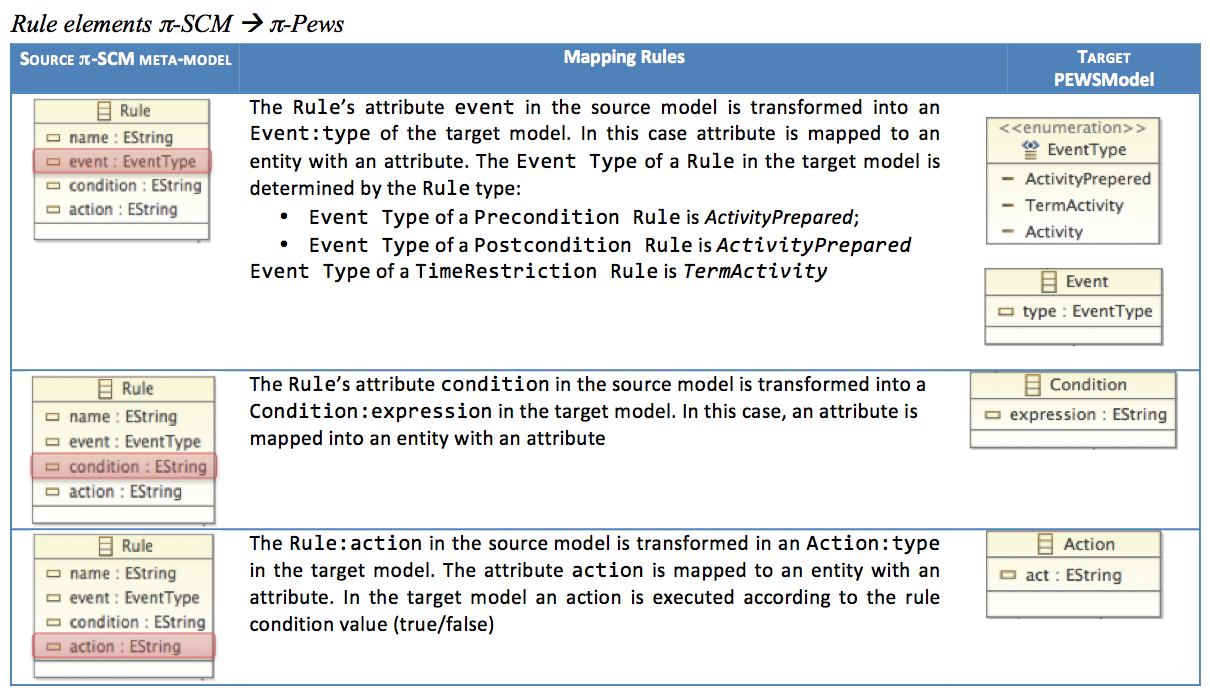
\includegraphics[width=0.96\textwidth]{figs/Mapping-1c.png}
}
\caption{ $\pi$-SCM to $\pi$-{\sc Pews} transformations (Rules).}
\label{fig:transformationsC}
\end{figure}


%*********************************************************************************************************

\section{Applying $\pi$-SOD-M: a case study}
4.1 Presentar los modelos para el caso y explicar las transformaciones
4.2 Discussion. (o Lecciones aprendidas del caso)

%Consider for instance the following scenario. An organization wants to provide the services' based application "To Publish Music" that monitors the music a person is listening during some periods of time and sends the song title  to this person's Twitter and Facebook accounts. Thus, this social network user will have her status synchronized in  Twitter and Facebook (i.e., either the same title is published in both accounts or it is not updated) with the title of the music she is listening in Spotify.
%For developing this services' based application it is necessary to compose the following services  calling  their  exported methods:
%\begin{itemize}
%\item The music service   Spotify exports a method for obtaining information  %about the music a given user is listening:
%%\begin{itemize} \item {\sf\small get-Last-Song ( userid ): String} ; %%\end{itemize}
%\item Facebook and Twitter services export a method for  updating the status of a given user:
%\begin{itemize} 
%%\item{\sf\small get-Status ( usedid ): String ; 
%\item {\sf\small update-Status ( userid, new-status ): String}; 
%\end{itemize}
%\end{itemize}
%
%Figure \ref{fig:E3valuemodel} shows the E3 value model \cite{e3value} of
%the scenario. The E3 value model is a business model that represents a business case graphically as a set of value exchanges ($\nabla$$\triangle$) and value activities (rounded boxes) performed by business actors (squared boxes) and allows us to understand the environment in which the services' composition will be placed. 
%The model in Figure \ref{fig:E3valuemodel} shows Spotify and a private application (which is also a service) that directly interact with users for providing free services for listening and publishing information about music being listened by users. The private application interacts with Spotify for obtaining free information about the flow of music being listened by a user in return of a fee (i.e., premium subscription). Finally, the private application interacts with Facebook and Twitter for updating the user's status and thereby they share non material benefits (i.e., the fact that users subscribe to their networks and are active on them thanks to the private application).

%Figure \ref{fig:E3valuemodel} shows the BPMN model  \footnote{Details on BPMN (Business Process Management Notation) can be found in http://www.bpmn.org/} of the scenario. 
%The "To Publish Music" scenario 
%%(showed by doted line) 
%starts by contacting the music service Spotify for retrieving the user's  musical status (activity {\sf Get Song}). 
%Twitter and Facebook services are then contacted in parallel for updating the user's status with the corresponding song title (activities {\sf Update Twitter} and {\sf Update Facebook}).
%\begin{figure}
%\centering
%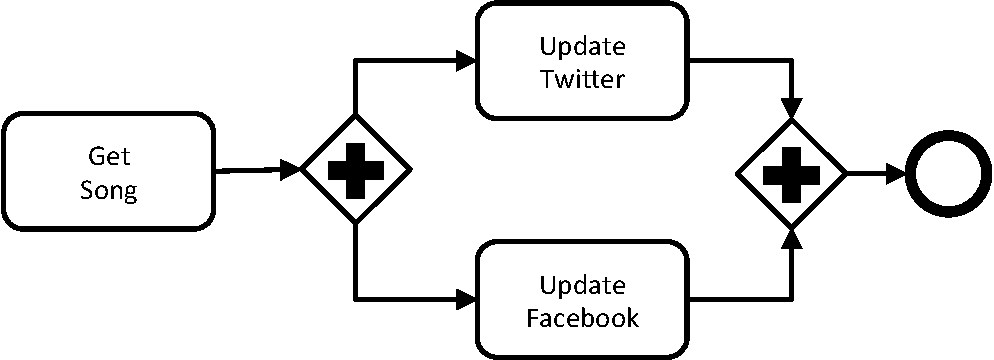
\includegraphics[width=0.55\textwidth]{figs/SC}
%\caption{BPMN model of the "To Publish Music" scenario}
%\label{fig:E3valuemodel}
%\end{figure}

In order to introduce the context of our work consider the Tracking crime application where civil population and by police share information about criminality in given zones of an imaginary city. 
Users signal crimes using twitter and police officers notify crimes  they have to deal with. 
Some of this information, if it is not confidential, can be shared to the community of users using this application. 
Users can track crimes in given zones and see information located in a map according to their privileges.  
For example civilians can ask Locate the crimes done the last month 100 km from my current position that happened between 8:00 and 14:00.
While police officers can ask Locate the regions in my sector where murders happened in the last month
This information can come from the police database and from twitter posts. 
The zones of the city are thereby according to their degree of criminality.

 In order to provide these functions the application benefits from existing services that provide information,  storage and data visualization functions. Thus, the application is a service based application that implements a business process.
 The business process is specified in terms of ordered tasks and define the application logic of a Service oriented Application. Tasks can be performed by a person or an entity. In our context, tasks are implemented by Services. 
Service is an application implemented by a provider that exports an API through a network (e.g., Internet)
API is defined using an interface definition language (IDL, e.g., WSDL for Web services).
 In our example the business procces can start with one of two tasks: Notify a crime, or track a crime. A notified crime can be then stored in a database. Tracked crimes are visualized in a map and then the used can ask for detailed information. They are implemented by four services: twitter and an adhoc police service for notifying crimes, Amazon as persistence service and google maps for visualizing and locating crimes in a map. 
Note that a task can be implemented by a service composition. This is the case of the task Notify crime in our example that enables to notify crimes through twitter or through the police notification service. 
 

Business processes have also associated rules and constraints that define their non functional requirements.  
NFR represents the “semantics” and the conditions in which the tasks must be done. 
In our example we have some constraints. 
\begin{itemize}
\item Twtter requires to be accessed through an authentication protocol, and the police crime notification service has a control  access protocol and allows only 3 tries to access it. 
\item Only users with enough privileges can store crimes’ notifications. 
\item Users can only track crimes notified by providers t that hey have authorization to contact; For example civil population cannot track all the crimes notified by the police. 
\item If the google map is unavailable the results of a track request are delivered on text. 
\item If a user tracks crimes that are provided by a service for which she does not have authorization then show an empty map. 
\item Detailed information about a crime depends on the user privileges, on the police assignment regions. 
\item The tracking crime app keeps track of the accesses to detailed information about crimes. 
\end{itemize}

Through the example we underlined that every application implements functional aspects that describe its application logic. Recall that an application logic refers to routines that perform the activities to reach the application objective.
Also there are non functional properties derived from NFR. They refer to strategies to be considered for the application execution like: security, isolation, adaptability, atomicity, and more.
These non functional properties must be ensured at execution time, and they are not completely defined within the application logic.

The challenge is to define them and to associate them with the application logic considering that different to existing solutions that suppose that it is possible to access the execution stat of all the components  of an application and that the application has complete control on them, in the case for service oriented applications  the components are autonomous services
API does not necessarily export information about methods dependency (e.g., in the REST protocol);
they do not share their state (stateless).






Given a set of services with their exported methods known in advance or provided by a  service directory, building services' based applications can be  a simple task that implies expressing an application logic as a services' composition. The challenge being  ensuring the compliance between the specification and the resulting application. Software engineering methods (e.g., \cite{1,2,decastro1,PapazoglouH06}) today can help to ensure this compliance, particularly when information systems include several sometimes complex business processes calling Web services or legacy applications exported as services. 

%..--..--..--..--..--..--..--..--..--..--..--..--..--..--..--..--..--..--..--..--..--..--..--..--..--..--..--..--..--..--..--..--..--..--..--..--..--..--
\subsection{Modeling a services' based application}
%..--..--..--..--..--..--..--..--..--..--..--..--..--..--..--..--..--..--..--..--..--..--..--..--..--..--..--..--..--..--..--..--..--..--..--..--..--..--
 Figure \ref{fig:sodm} shows  SOD-M that defines a service oriented approach   providing  a set of guidelines to build services' based information systems (SIS) \cite{decastro1,decastro2}.  Therefore, SOD-M proposes to use services as first-class objects for the whole process of the SIS  development and it  follows a Model Driven Architecture (MDA) \cite{miller}  approach. Extending from the highest level of abstraction of the MDA, SOD-M provides  a conceptual structure to: first, capture the system requirements and specification in high-level abstraction models (computation independent models, CIMÕs); next,  starting from such models build platform independent models (PIMÕs) specifying the system details; next transform such models into platform specific models (PSMÕs) that bundles the specification of the system with the details of the targeted platform; and finally, serialize such model into the working-code that implements the system. 
\begin{figure} [htpb]
\centering
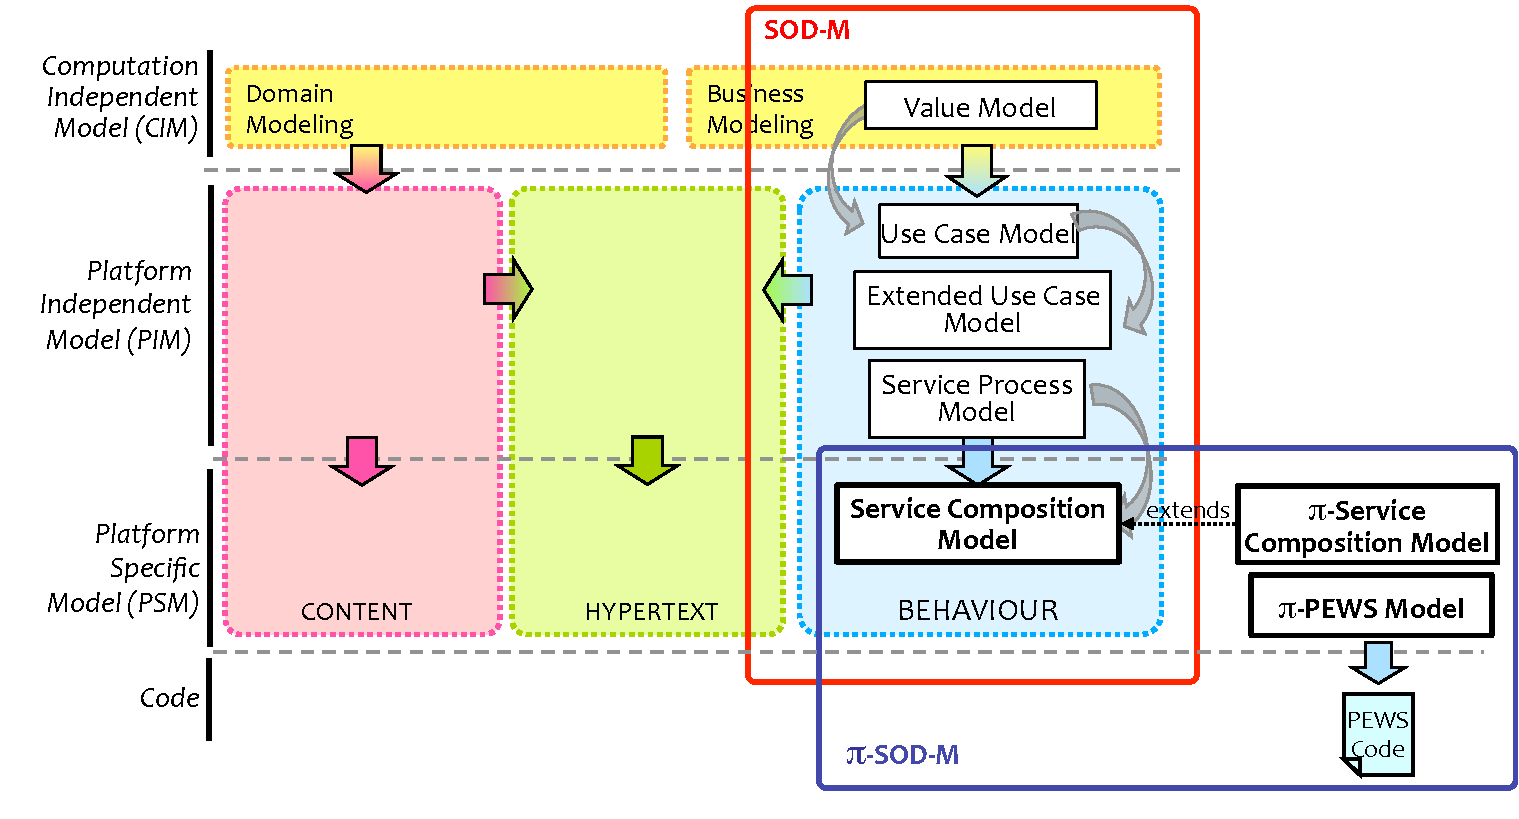
\includegraphics[width=0.65\textwidth]{figs/SODM}
\caption{SOD-M development process}
\label{fig:sodm}
\end{figure} 
As shown in Figure \ref{fig:sodm}, the SOD-M model-driven process begins by building the high-level computational independent models and enables specific models for a service platform to be obtained as a result  \cite{decastro1}. Referring to the "To Publish Music" application, using SOD-M the designer starts defining an E3value model \footnote{The E3 value model is a business model that represents a business case %graphically as a set of value exchanges ($\nabla$$\triangle$) and value activities (rounded boxes) performed by business actors (squared boxes) 
and allows  to understand the environment in which the services' composition will be placed \cite{e3value}.}  at the CIM level and then the corresponding models of the PIM are generated leading to a services' composition model (SCM).
%SOD-M proposes a set of models, :  i) the three different MDA abstraction levels: CIM, PIM and PSM; and ii) SOD-M views: business and information system views. 
%Model-Driven Engineering (MDE) \cite{schmidt} and particularly MDA \footnote{Model Driven Architecture (MDA)  is the particular model-driven proposal defined by the Object Management Group (OMG).} 
%provide
%is an evolving approach to software development that deals with the provision of 
%models, transformations between them and code generators to address software development. 
%One of the main advantages of model-driven approaches is the provision of 
%It also provides a conceptual structure where the models used by business managers and analysts can be traced towards more detailed models used by software developers.  

%Now, consider that besides the services' composition that represents the order in which the services are called for implementing the application "To Publish Music" it is necessary to model  other requirements that represent the (i) conditions imposed by services for being contacted, for example the fact the Facebook and Twitter require authentication protocol in order to call their methods for updating the wall; (ii) the conditions stemming from the business rules of the application logic, for example the fact that the walls in Facebook and Twitter must show the same song title and if this is not possible then none of them is updated. 

%..--..--..--..--..--..--..--..--..--..--..--..--..--..--..--..--..--..--..--..--..--..--..--..--..--..--..--..--..--..--..--..--..--..--..--..--..--..--
\subsection{Modeling non-functional constraints of services' based applications}
%..--..--..--..--..--..--..--..--..--..--..--..--..--..--..--..--..--..--..--..--..--..--..--..--..--..--..--..--..--..--..--..--..--..--..--..--..--..--
Adding non-functional requirements and services constraints in the services' composition is a complex task that implies programming  protocols for instance authentication protocols to call a service in our example, and atomicity (exception handling and recovery) for ensuring a true synchronization of the results produced by the service methods calls.
% song title disseminated in the walls of the user's Facebook and Twitter accounts. 

Service oriented computing promotes ease of information systems' construction thanks, for instance, to services' reuse. Yet, this is not applied to non-functional constraints as the ones described previously, because they do not follow in general the same service oriented principle and because they are often not fully considered in the specification process of existing services' oriented development methods. Rather, they   are either supposed to be ensured by the underlying execution platform, or they are programmed through ad-hoc protocols. Besides,  they are partially or rarely methodologically derived from the application specification, and they are added once the code has been implemented. In consequence, the resulting application does not fully preserve the compliance and reuse expectations provided by the service oriented computing methods.

%..--..--..--..--..--..--..--..--..--..--..--..--..--..--..--..--..--..--..--..--..--..--..--..--..--..--..--..--..--..--..--..--..--..--..--..--..--..--
%\subsection{$\pi$-SOD-M}
%..--..--..--..--..--..--..--..--..--..--..--..--..--..--..--..--..--..--..--..--..--..--..--..--..--..--..--..--..--..--..--..--..--..--..--..--..--..--

%
%Our proposal, called $\pi$-SOD-M, extends the services' composition model of the SOD-M method  with the notion of {\em A-Policy} \cite{Espinosa-Oviedo2011a} for representing services' composition constraints. 
%
Our work extends SOD-M for building applications by modeling the application logic and its associated non-functional constraints and thereby ensuring the generation of reliable services' composition. 
%This method is described in the following sections.
In order to do, our work organizes non-functional constraints into 
three layers representing: application modeling, services composition and services. The service composition layer serves as an integration layer between the services layer that exports methods and has associated constraints and characteristics; and the application layer that expresses requirements.
At the application layer NFP can refer to business rules and values. A value NFR expresses constraints about the way data and functions can be accessed and executed. For example accessing methods under security protocols.

Business NFP at the service layer concerns properties that are associated to services and defines how to call their exported operations (business properties). For example, response time, storage capacity (e.g., Dropbox service provides 5Giga free storage). Value constraints concern more on the conditions in which services can be used. For example, accessing to a function within an authentica-tion protocol.

Finally, at the service composition layer gives an abstract view of the kind of properties exported by services that can be combined for providing NFP for a composition. For example, confidentiality, authentication, privacy and access control can provide security at the service composition layer.

As a first step in our approach,  we started modeling non-functional constraints at the PSM level. Thus, in this paper we  propose the $\pi$-SCM, the services' composition meta-model extended with {\em A-policies} for modeling non-functional constraints (highlighted in Figure  \ref{fig:sodm} and described in Section \ref{sec:piscm}).  $\pi$-SOD-M defines the $\pi$-{\sc Pews}  meta-model providing guidelines for expressing the services' composition and the {\em A-policies} (see Section \ref{sec:pewsmetamodel}), and also defines model to model transformation rules for generating  $\pi$-{\sc Pews} models starting from $\pi$-SCM models that will support executable code generation (see Section \ref{sec:mmrules}). Finally, our work defines model to text transformation rules for generating the program that implements both the services' composition and the associated {\em A-policies} and that is executed by an adapted engine (see Section \ref{sec:implementation}).





%*********************************************************************************************************
\section{Conclusions and future work}\label{sec:conclusions}
This paper presented \pisodm for designing and developing reliable service-based applications. 
\pisodm is an MDA methodology that extends a previously defined method (called SOD-M) to include Non-Functional Requirements.
These requirements are taken into account from the initial stages of the software development process.
Non-functional constraints are related to business rules associated to the behavior of the application and, in the case of service-based applications, they are also concerned with constraints imposed by the services. 

Our methodology includes two CIM-level models, three PIM-level models and one PSM-level model. 
We implemented the meta-models on the Eclipse platform and we validated the approach by using an industrially inspired use case.

Our case study demonstrates the applicability of \pisodm.
The case study was developed together with our industrial partner, GCP Global.
The Company is using \pisodm for the development of their product.
The case study presented here is a simplified version of their application.
%*********************************************************************************************************


\appendix

%*********************************************************************************************************
\section{Implementation issues}\label{sec:implementation}

This section  describes the $\pi$-SOD-M development environment that implements the generation of {\em A-policies}' based services' compositions. For a given services' based application, the process  consists in generating the  code starting from a $\pi$-SCM modeling an application. Note that the services' composition model is not modeled from scratch, but it is the result of a general process defined by the $\pi$-SOD-M method in which a set of models are built following a service oriented approach \cite{decastro1}.

%We used the Eclipse Modeling Framework (EMF) to implement the whole model transformation process \footnote {The EMF project is a modeling framework and code generation facility for building tools and other applications based on a structured data model.}. From a model specification described in XMI, EMF provides tools and runtime support to produce a set of Java classes for the model, along with a set of adapter classes that enable viewing and command-based editing of the model, and a basic editor.
%In order to automate the transformation we specified  transformation rules using the ATL model transformation language Finally, in order to generate code we  used Acceleo \footnote{http://www.acceleo.org/pages/home/en}.

%..--..--..--..--..--..--..--..--..--..--..--..--..--..--..--..--..--..--..--..--..--..--..--..--..--..--..--..--..--..--..--..--..--..--..--..--..--..--
\subsection{$\pi$-SOD-M Development Environment}
%..--..--..--..--..--..--..--..--..--..--..--..--..--..--..--..--..--..--..--..--..--..--..--..--..--..--..--..--..--..--..--..--..--..--..--..--..--..--

Figure \ref{fig:policymanager} depicts a general architecture of the $\pi$-SOD-M Development Environment showing the set of plug-ins  developed in order to implement it. The environment implements the abstract architecture shown in Figure \ref{fig:sodm}. Thus, it consists of plug-ins implementing the $\pi$-SCM and $\pi$-{\sc Pews} meta-models used for defining models specifying services' compositions and their associated policies; and ATL rules for transforming  PSM models (model to model transformation) and finally generating code (model to text transformation).
\begin{figure}[htpb]
	\begin{center}
		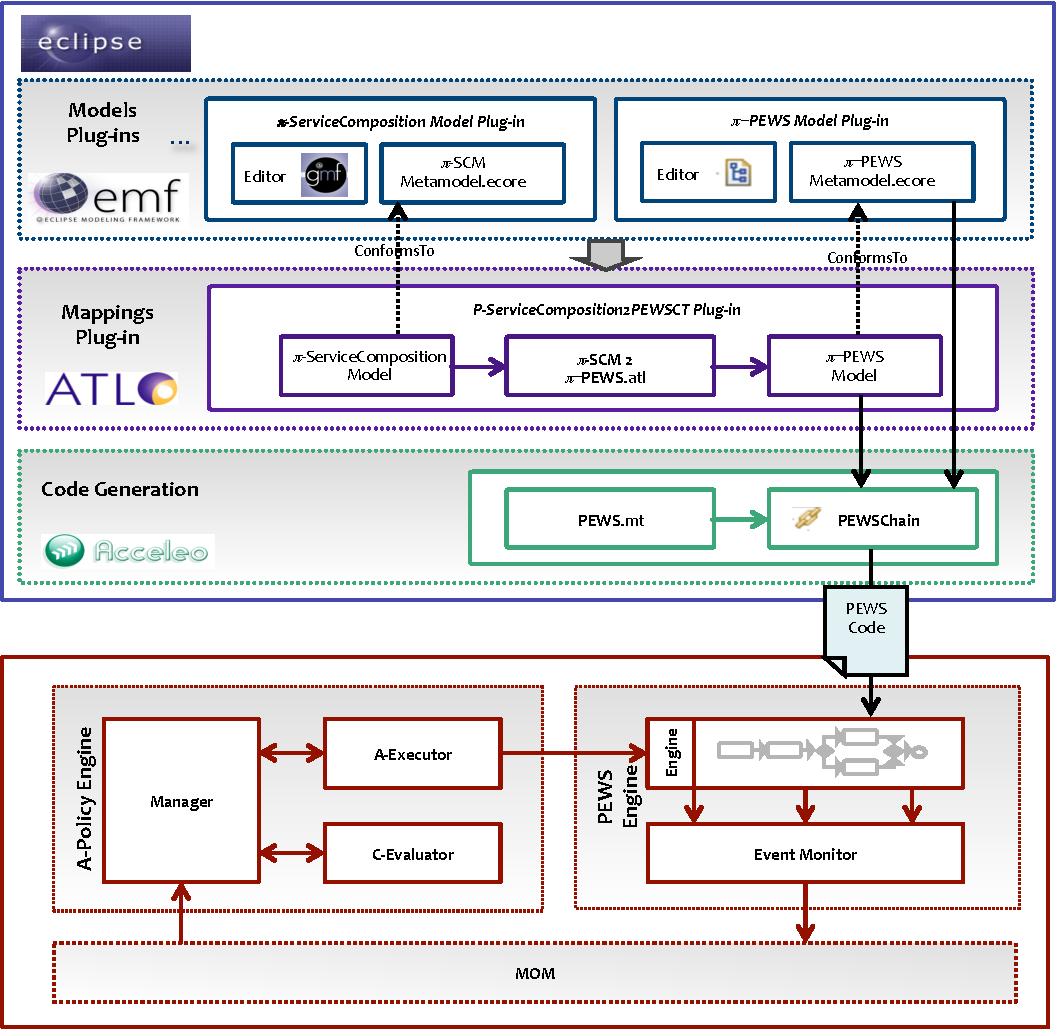
\includegraphics[width=0.60\textwidth]{figs/architecture}
	\end{center}
		\caption{$\pi$-SOD-M Development Environment}
   \label{fig:policymanager}
\end{figure}
\begin{itemize}
\item 	We  used the Eclipse Modeling Framework (EMF) \footnote {The EMF project is a modeling framework and code generation facility for building tools and other applications based on a structured data model.}   for implementing the meta-models  $\pi$- SCM and $\pi$-{\sc Pews}. Then, starting form these meta-models, we  developed the models' plug-ins needed to support the graphical representation of the $\pi$- SCM and $\pi$-{\sc Pews} models ($\pi$-ServiceCompostion Model and $\pi$-PEWS Model plug-ins).

\item	 We used  ATL \footnote{http://eclipse.org/atl/. An ATL program is basically a set of rules that define how source model elements are matched and navigated to create and initialize the elements of the target models.}
for  developing the mapping plug-in implementing the  mappings between models ($\pi$-ServiceComposition2$\pi$-PEWS Plug-in).

\item 	We  used Acceleo \footnote{http://www.acceleo.org/pages/home/en} for implementing  the code generation plug-in. We coded the pews.mt program  that implements the model to text transformation for generating executable code. It takes as input a $\pi$-PEWS model implementing a specific services' composition and it generates the code to be executed by the 
{\em A-policy} based services' composition execution environment. 

%\item Finally, we created a chain execution  to execute the model to text transformation.
\end{itemize}
%
%
%

%
As  shown in Figure \ref{fig:policymanager}, once an instance of a PEWS code is obtained starting form a particular $\pi$-services' composition model it can be executed over {\em A-policy} based services' composition execution environment  consisting of a composition engine and a {\em A-policy} manager.  The  {\em A-policy} manager  consists of three main components Manager, for scheduling the execution of rules, C-Evaluator and A-Executor respectively for evaluating rules' conditions and executing their actions. The {\em A-policy} Manager interacts with a composition engine thanks to a  message communication layer (MOM).


The composition engine manages the life cycle of the composition. Once a composition instance is activated, the engine schedules the composition activities according to the composition control flow.
Each activity is seen as the process where the service method call is executed.
The execution of an activity has four states: prepared, started, terminated, and failure.
The execution of the control flow (sequence, and/or split and join) can also be prepared, started, terminated and raise a failure.

At execution time, the evaluation of policies done by the {\em A-policy} manager must be synchronized with the execution of the services' composition (i.e., the execution of an activity or a control flow).  Policies associated to a scope are activated when the execution of its scope starts. A {\em A-policy} will have to be executed only if one or several of its rules is triggered. If several rules are triggered the {\em A-policy} manager first builds an execution plan that specifies the order in which such rules will be executed according to the strategies defined in the following section. 
%Once rules have been executed, the {\em A-policy} finishes its execution and returns to a sleeping state.
If rules belonging to several policies are triggered then policies are also ordered according to an execution plan. The execution of policies is out of the scope of this paper, the interested reader can refer to \cite{Espinosa-Oviedo2011a} for further details.
%The order of policies has implications on the global order of the rules to be executed.

%..--..--..--..--..--..--..--..--..--..--..--..--..--..--..--..--..--..--..--..--..--..--..--..--..--..--..--..--..--..--..--..--..--..--..--..--..--..--
\subsection{Validation}
%..--..--..--..--..--..--..--..--..--..--..--..--..--..--..--..--..--..--..--..--..--..--..--..--..--..--..--..--..--..--..--..--..--..--..--..--..--..--

We validated our approach  by implementing the "To Publish Music" application. It consists in atomically synchronizing  the status of a user's accounts according to the music she listens in Spotify and using authentication protocols for updating the walls' status in her Facebook and Twitter accounts.  Once the services' composition model has been annotated with the corresponding policies, then the reliable composition code can be generated using the rules defined for this purpose. Our implementation includes a  code generator that generates executable code for a reliable services' composition.
The model represents an services' composition expression and its associated policies. 


We tested the application  in order to see whether the coordination tolerated services unavailability keeping the status synchronized. Particularly, the token of the activity associated to Twitter was consistently obtained when the service was available. We also implemented a reference coordination without policies. We dealt with the availability exceptions by hand and the authentication protocols were embedded within the activities code. During our validation Twitter changed the authentication protocol and the maintenance of the application this implied re-programming the reference application. Instead, with the policies approach we only had to desactivate the corresponding policy and associate the appropriate one to the activity calling the service Twitter (one code line), and run the application again.


%*********************************************************************************************************



%% The Appendices part is started with the command \appendix;
%% appendix sections are then done as normal sections
%% \appendix

%% \section{}
%% \label{}

%% References
%%
%% Following citation commands can be used in the body text:
%% Usage of \cite is as follows:
%%   \cite{key}          ==>>  [#]
%%   \cite[chap. 2]{key} ==>>  [#, chap. 2]
%%   \citet{key}         ==>>  Author [#]

%% References with bibTeX database:

\bibliographystyle{plain}
\bibliography{biblio}

%% Authors are advised to submit their bibtex database files. They are
%% requested to list a bibtex style file in the manuscript if they do
%% not want to use model1a-num-names.bst.

%% References without bibTeX database:

% \begin{thebibliography}{00}

%% \bibitem must have the following form:
%%   \bibitem{key}...
%%

% \bibitem{}

% \end{thebibliography}

\end{document}

%%
%% End of file `elsarticle-template-1a-num.tex'.
